\documentclass{article}\usepackage[T1]{fontenc}\usepackage{tikz,float,esint}\usetikzlibrary{arrows.meta,calc}
\begin{document}
\begin{figure}[H]
\centering
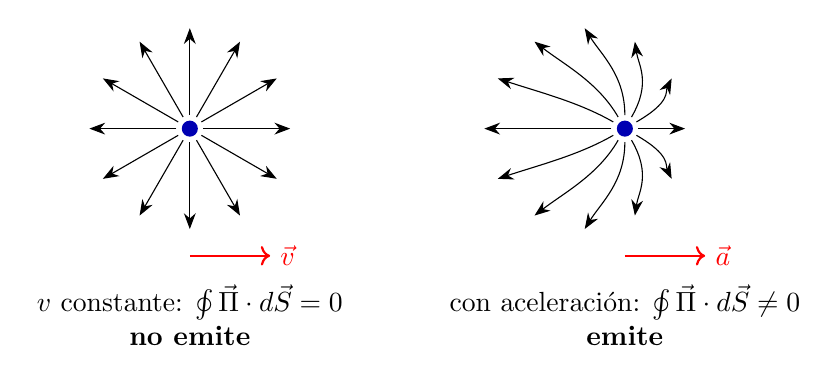
\begin{tikzpicture}[scale=0.85]
  % carga con v constante
  \begin{scope}
    \fill[blue!70!black] (0,0) circle (0.12);
    \foreach \a in {0,30,...,330}
      \draw[-{Stealth[length=2mm]}] (\a:0.2) -- (\a:1.5);
    \draw[->,thick,red] (0,-1.9) -- (1.2,-1.9) node[right]{$\vec v$};
    \node at (0,-2.6) {$v$ constante: $\oint\vec\Pi\cdot d\vec S=0$};
    \node at (0,-3.1) {\textbf{no emite}};
  \end{scope}
  % carga acelerada
  \begin{scope}[xshift=6.5cm]
    \fill[blue!70!black] (0,0) circle (0.12);
    \foreach \a in {0,30,...,330}
      \draw[-{Stealth[length=2mm]}] (\a:0.2) .. controls (\a:0.8) and ($(\a:1.1)+(-0.35,0)$) .. ($(\a:1.5)+(-0.6,0)$);
    \draw[->,thick,red] (0,-1.9) -- (1.2,-1.9) node[right]{$\vec a$};
    \node at (0,-2.6) {con aceleración: $\oint\vec\Pi\cdot d\vec S\neq0$};
    \node at (0,-3.1) {\textbf{emite}};
  \end{scope}
\end{tikzpicture}
\caption{Líneas de campo de una carga con velocidad constante (los campos se mueven con la carga) y de una carga acelerada (las líneas se curvan).}
\end{figure}
\end{document}
